% Options for packages loaded elsewhere
\PassOptionsToPackage{unicode}{hyperref}
\PassOptionsToPackage{hyphens}{url}
%
\documentclass[
]{article}
\usepackage{lmodern}
\usepackage{amssymb,amsmath}
\usepackage{ifxetex,ifluatex}
\ifnum 0\ifxetex 1\fi\ifluatex 1\fi=0 % if pdftex
  \usepackage[T1]{fontenc}
  \usepackage[utf8]{inputenc}
  \usepackage{textcomp} % provide euro and other symbols
\else % if luatex or xetex
  \usepackage{unicode-math}
  \defaultfontfeatures{Scale=MatchLowercase}
  \defaultfontfeatures[\rmfamily]{Ligatures=TeX,Scale=1}
\fi
% Use upquote if available, for straight quotes in verbatim environments
\IfFileExists{upquote.sty}{\usepackage{upquote}}{}
\IfFileExists{microtype.sty}{% use microtype if available
  \usepackage[]{microtype}
  \UseMicrotypeSet[protrusion]{basicmath} % disable protrusion for tt fonts
}{}
\makeatletter
\@ifundefined{KOMAClassName}{% if non-KOMA class
  \IfFileExists{parskip.sty}{%
    \usepackage{parskip}
  }{% else
    \setlength{\parindent}{0pt}
    \setlength{\parskip}{6pt plus 2pt minus 1pt}}
}{% if KOMA class
  \KOMAoptions{parskip=half}}
\makeatother
\usepackage{xcolor}
\IfFileExists{xurl.sty}{\usepackage{xurl}}{} % add URL line breaks if available
\IfFileExists{bookmark.sty}{\usepackage{bookmark}}{\usepackage{hyperref}}
\hypersetup{
  hidelinks,
  pdfcreator={LaTeX via pandoc}}
\urlstyle{same} % disable monospaced font for URLs
\usepackage{color}
\usepackage{fancyvrb}
\newcommand{\VerbBar}{|}
\newcommand{\VERB}{\Verb[commandchars=\\\{\}]}
\DefineVerbatimEnvironment{Highlighting}{Verbatim}{commandchars=\\\{\}}
% Add ',fontsize=\small' for more characters per line
\newenvironment{Shaded}{}{}
\newcommand{\AlertTok}[1]{\textcolor[rgb]{1.00,0.00,0.00}{\textbf{#1}}}
\newcommand{\AnnotationTok}[1]{\textcolor[rgb]{0.38,0.63,0.69}{\textbf{\textit{#1}}}}
\newcommand{\AttributeTok}[1]{\textcolor[rgb]{0.49,0.56,0.16}{#1}}
\newcommand{\BaseNTok}[1]{\textcolor[rgb]{0.25,0.63,0.44}{#1}}
\newcommand{\BuiltInTok}[1]{#1}
\newcommand{\CharTok}[1]{\textcolor[rgb]{0.25,0.44,0.63}{#1}}
\newcommand{\CommentTok}[1]{\textcolor[rgb]{0.38,0.63,0.69}{\textit{#1}}}
\newcommand{\CommentVarTok}[1]{\textcolor[rgb]{0.38,0.63,0.69}{\textbf{\textit{#1}}}}
\newcommand{\ConstantTok}[1]{\textcolor[rgb]{0.53,0.00,0.00}{#1}}
\newcommand{\ControlFlowTok}[1]{\textcolor[rgb]{0.00,0.44,0.13}{\textbf{#1}}}
\newcommand{\DataTypeTok}[1]{\textcolor[rgb]{0.56,0.13,0.00}{#1}}
\newcommand{\DecValTok}[1]{\textcolor[rgb]{0.25,0.63,0.44}{#1}}
\newcommand{\DocumentationTok}[1]{\textcolor[rgb]{0.73,0.13,0.13}{\textit{#1}}}
\newcommand{\ErrorTok}[1]{\textcolor[rgb]{1.00,0.00,0.00}{\textbf{#1}}}
\newcommand{\ExtensionTok}[1]{#1}
\newcommand{\FloatTok}[1]{\textcolor[rgb]{0.25,0.63,0.44}{#1}}
\newcommand{\FunctionTok}[1]{\textcolor[rgb]{0.02,0.16,0.49}{#1}}
\newcommand{\ImportTok}[1]{#1}
\newcommand{\InformationTok}[1]{\textcolor[rgb]{0.38,0.63,0.69}{\textbf{\textit{#1}}}}
\newcommand{\KeywordTok}[1]{\textcolor[rgb]{0.00,0.44,0.13}{\textbf{#1}}}
\newcommand{\NormalTok}[1]{#1}
\newcommand{\OperatorTok}[1]{\textcolor[rgb]{0.40,0.40,0.40}{#1}}
\newcommand{\OtherTok}[1]{\textcolor[rgb]{0.00,0.44,0.13}{#1}}
\newcommand{\PreprocessorTok}[1]{\textcolor[rgb]{0.74,0.48,0.00}{#1}}
\newcommand{\RegionMarkerTok}[1]{#1}
\newcommand{\SpecialCharTok}[1]{\textcolor[rgb]{0.25,0.44,0.63}{#1}}
\newcommand{\SpecialStringTok}[1]{\textcolor[rgb]{0.73,0.40,0.53}{#1}}
\newcommand{\StringTok}[1]{\textcolor[rgb]{0.25,0.44,0.63}{#1}}
\newcommand{\VariableTok}[1]{\textcolor[rgb]{0.10,0.09,0.49}{#1}}
\newcommand{\VerbatimStringTok}[1]{\textcolor[rgb]{0.25,0.44,0.63}{#1}}
\newcommand{\WarningTok}[1]{\textcolor[rgb]{0.38,0.63,0.69}{\textbf{\textit{#1}}}}
\usepackage{longtable,booktabs}
% Correct order of tables after \paragraph or \subparagraph
\usepackage{etoolbox}
\makeatletter
\patchcmd\longtable{\par}{\if@noskipsec\mbox{}\fi\par}{}{}
\makeatother
% Allow footnotes in longtable head/foot
\IfFileExists{footnotehyper.sty}{\usepackage{footnotehyper}}{\usepackage{footnote}}
\makesavenoteenv{longtable}
\usepackage{graphicx}
\makeatletter
\def\maxwidth{\ifdim\Gin@nat@width>\linewidth\linewidth\else\Gin@nat@width\fi}
\def\maxheight{\ifdim\Gin@nat@height>\textheight\textheight\else\Gin@nat@height\fi}
\makeatother
% Scale images if necessary, so that they will not overflow the page
% margins by default, and it is still possible to overwrite the defaults
% using explicit options in \includegraphics[width, height, ...]{}
\setkeys{Gin}{width=\maxwidth,height=\maxheight,keepaspectratio}
% Set default figure placement to htbp
\makeatletter
\def\fps@figure{htbp}
\makeatother
\setlength{\emergencystretch}{3em} % prevent overfull lines
\providecommand{\tightlist}{%
  \setlength{\itemsep}{0pt}\setlength{\parskip}{0pt}}
\setcounter{secnumdepth}{-\maxdimen} % remove section numbering

\author{}
\date{}

\begin{document}

\hypertarget{deep-learning}{%
\section{Deep Learning}\label{deep-learning}}

My deep learning notes

\hypertarget{terminology}{%
\subsection{Terminology}\label{terminology}}

\begin{longtable}[]{@{}cc@{}}
\toprule
Term & Definition\tabularnewline
\midrule
\endhead
ANN & Artificial Neural Network\tabularnewline
Layer & Organized Neurons\tabularnewline
Deep Network & A Network with more than one hidden layer\tabularnewline
Activation Function & Non linear function that follows a dense
layer\tabularnewline
\bottomrule
\end{longtable}

\hypertarget{other-notes}{%
\subsubsection{Other notes}\label{other-notes}}

model = net = neural network

neuron = node

\hypertarget{layers}{%
\subsection{Layers}\label{layers}}

Layers are organized neurons.

Layers are sperated into 3 catagories

\begin{itemize}
\tightlist
\item
  An input layer
\item
  one or more hidden layers
\item
  An output layer
\end{itemize}

Here is an image visualizing a network with s input layer made of 3
neurons, 1 hidden layer made up of 4 neurons, and a output layer made
out of 2 neurons.

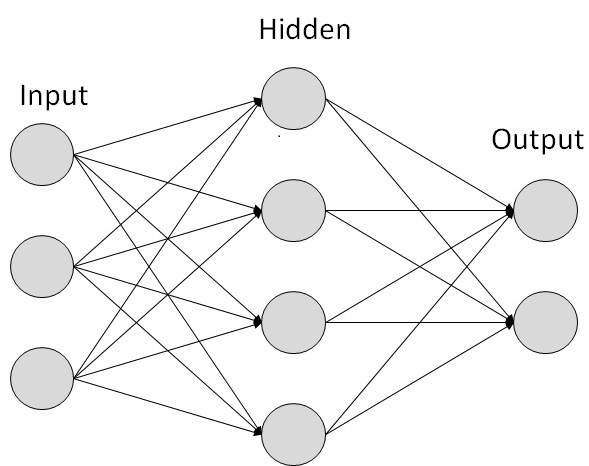
\includegraphics{images/neural-net.jpg}

Differnt layers will perform differnt operations on data. Data flows
from the input layer through the hidden layers until the output layer is
reached.

How many neurons should I assign to each layer?

\begin{longtable}[]{@{}cc@{}}
\toprule
Type & How to allocate\tabularnewline
\midrule
\endhead
Input & One neuron for each component of input data\tabularnewline
Hidden & Arbitrarily Chosen\tabularnewline
Output & One node for each of the possible desired
outcomes\tabularnewline
\bottomrule
\end{longtable}

So how would we implement such a network in Keras? The following is a
Keras implementation of the Neural network above

\begin{Shaded}
\begin{Highlighting}[]
\ImportTok{from}\NormalTok{ keras.models }\ImportTok{import}\NormalTok{ Sequential}
\ImportTok{from}\NormalTok{ keras.layers }\ImportTok{import}\NormalTok{ Dense}

\NormalTok{model }\OperatorTok{=}\NormalTok{ Sequential([}
\NormalTok{    Dense(}\DecValTok{4}\NormalTok{, input\_shape}\OperatorTok{=}\NormalTok{(}\DecValTok{3}\NormalTok{,)),}
\NormalTok{    Dense(}\DecValTok{2}\NormalTok{)}
\NormalTok{])}
\end{Highlighting}
\end{Shaded}

The output of one layer is then passed to another and another, and soo
on the output is computed with the following equation.

\begin{Shaded}
\begin{Highlighting}[]
\NormalTok{output }\OperatorTok{=}\NormalTok{ activation(}\BuiltInTok{sum}\NormalTok{(weights))}
\end{Highlighting}
\end{Shaded}

this process is repeated over and over untill we reach the output layer.
During this process weights will mutate in order to acheive optimized
weighting for each connection. This is known as a foward pass.

\hypertarget{activation-function}{%
\subsubsection{Activation Function}\label{activation-function}}

A activation function of a neuron defines the output of the specified
neuron given a set of inputs. Follows a layer.

Here are some exmaples of activation functions

\hypertarget{sigmoid}{%
\paragraph{Sigmoid}\label{sigmoid}}

\paragraph{Formula}

\[sigmoid(x) = \dfrac{e^x}{e^x+1}\]

Python code

\begin{Shaded}
\begin{Highlighting}[]
\ImportTok{from}\NormalTok{ math }\ImportTok{import}\NormalTok{ e}

\KeywordTok{def}\NormalTok{ sigmoid(x):}
    \ControlFlowTok{return}\NormalTok{ e}\OperatorTok{**}\NormalTok{x }\OperatorTok{/}\NormalTok{ e}\OperatorTok{**}\NormalTok{(x}\OperatorTok{+}\DecValTok{1}\NormalTok{) }
\end{Highlighting}
\end{Shaded}

\hypertarget{example}{%
\subsubsection{Example}\label{example}}

Say we have a program that we want to identify if the image is of a cat
or a dog. We would have 2 output nodes One representing a cat. And the
other a dog.

\hypertarget{keras}{%
\section{Keras}\label{keras}}

Keras is a simple API for describing neural networks

\hypertarget{layers-1}{%
\subsection{Layers}\label{layers-1}}

\hypertarget{dense}{%
\subsubsection{Dense}\label{dense}}

This is the most basic layer in a neural network. It connects it's
inputs to it's outputs. This layer merely connects inputs to outputs
within it's layer.

\hypertarget{convolutional}{%
\subsubsection{Convolutional}\label{convolutional}}

Used for work with images

\hypertarget{recurrent}{%
\subsubsection{Recurrent}\label{recurrent}}

Used for work with time series data.

\hypertarget{the-sequential-model}{%
\subsection{The Sequential Model}\label{the-sequential-model}}

The sequential Model is a linear stack of layers i.e.

\begin{Shaded}
\begin{Highlighting}[]
\CommentTok{\# Import the Sequential Model}
\ImportTok{from}\NormalTok{ keras.models }\ImportTok{import}\NormalTok{ Sequential}

\NormalTok{model }\OperatorTok{=}\NormalTok{ Sequential([}
\NormalTok{    Dense(}\DecValTok{32}\NormalTok{, input\_shape}\OperatorTok{=}\NormalTok{(}\DecValTok{10}\NormalTok{,), activation}\OperatorTok{=}\StringTok{\textquotesingle{}relu\textquotesingle{}}\NormalTok{),}
\NormalTok{    Dense(}\DecValTok{2}\NormalTok{, activation}\OperatorTok{=}\StringTok{\textquotesingle{}softmax\textquotesingle{}}\NormalTok{)}
\NormalTok{])}
\end{Highlighting}
\end{Shaded}


\end{document}
